
\section{Evaluation}
\label{sec:eval}

%In this section we evaluate various aspects of iProbe. Initially, we show the overhead of iProbe on SPEC CPU 2006 benchmarks\cite{specCPU2006}, we then showcase iProbe vs a normal mode, the binary generated with initial -finstrument-function flag, and the ColdPatched version of the same binary. Since iProbe is also geared towards monitoring large scale systems, we also show the overhead of iProbe "ColdPatched" binaries in terms of throughput in apache httpd server, and the mysql database. Then we present the overhead for "HotPatching" itself wherein we measure the time taken by iProbe to patch the functions in a live session. Lastly, we compare scalability of iProbe compared to existing state of the art technique SystemTap \cite{systemtap}

\subsection{Overhead of ColdPatch}
The SPEC INT CPU benchmarks 2006 \cite{specCPU2006} is a widely used benchmark in academia, industry and research as relevant representation of real world applications. 
We tested iProbe on 8 benchmark applications shown in Figure \ref{fig:overhead_table}. The first column shows the execution of a normal binary compiled without any instrumentation or debug flags. 
The next column shows the execution time of the corresponding binary compiled using the instrumentation flags (Note here the instrumentation functions are dummy functions). 
Lastly, we show the overhead of a ColdPatched iProbe binary with \texttt{NOP} instead of the call instruction. 
Each benchmark application was executed ten times using SPEC benchmark tools. 
The overhead for a ColdPatched binary was found to be less than five percent for all applications executed, and 0-2 percent for four of the benchmarks. 
The overhead here is basically because of the \texttt{NOP} instructions that are placed in the binary as place-holders for the HotPatching. 
In most non-compute intensive applications (e.g., apache, mysql) we have observed the overhead to be negligible (less than one percent), with no observable effect in terms of throughput. 
Further reduction of the overhead can be achieved by reducing the scope of the functions which are prepared for function tracing by iProbe; for example only using place holders in selected components that need to be further inspected. 
Negligible overhead of ColdPatching process of iProbe shows that applications can be prepared for instrumentation (HotPatching) without adversly effecting the usage of the application.
%Above add details on how components can be selected using -finstrument-functions-execlude-list/ compiler options

%A ColdPatched version of the apache httpd server was tested using the apache ab benchmarking tool, and the overhead was found to be less than 1 percent in throughput. We also ran iProbe on a ColdPatched version of mysql and found similar results. In section.\ref{sec:casestudy_mysql} we further discuss the use of iProbe in a practical debugging case scenario.

%In summary we could observe iProbe having a small to negligible overhead when running a ColdPatched binary. While the overhead of iProbe can be further reduced by using further optimizations in writing the patches, we believe this to be largely an acceptable overhead to enable long term monitoring of applications at the user-level. 


%\begin{table}[h]
%\begin{center}
%    \begin{tabular}{ | l | l | l | l|}
%    \hline
%    Name & Normal & Finstrument & ColdPatch \\ \hline
%    bzip2 & 30.7 & 31.2 & 30.7 \\ \hline
%    sjeng & 13.8 & 15.4 & 14.4 \\ \hline
%    perlbench & 5.24 & 5.49 & 5.24 \\ \hline
%    mcf & 5.98 & 6.72 & 6.28 \\ \hline
%    hmmer & 19.7 & 20 & 19.7  \\ \hline
%    gobmk & 53.4 & 56.6 & 55.5 \\ \hline
%    h264ref & 76.3 & 81 & 80.6 \\ \hline
%    astar & 32.6 & 41.6 & 34.3  \\ \hline
%    \end{tabular}
%\end{center}
%\label{tab:overhead_table}
%\caption{Overhead of iProbe "ColdPatch stage" on SPEC CPU 2006 benchmarks}
%\end{table}


\begin{figure}[h!]
  \begin{center}
    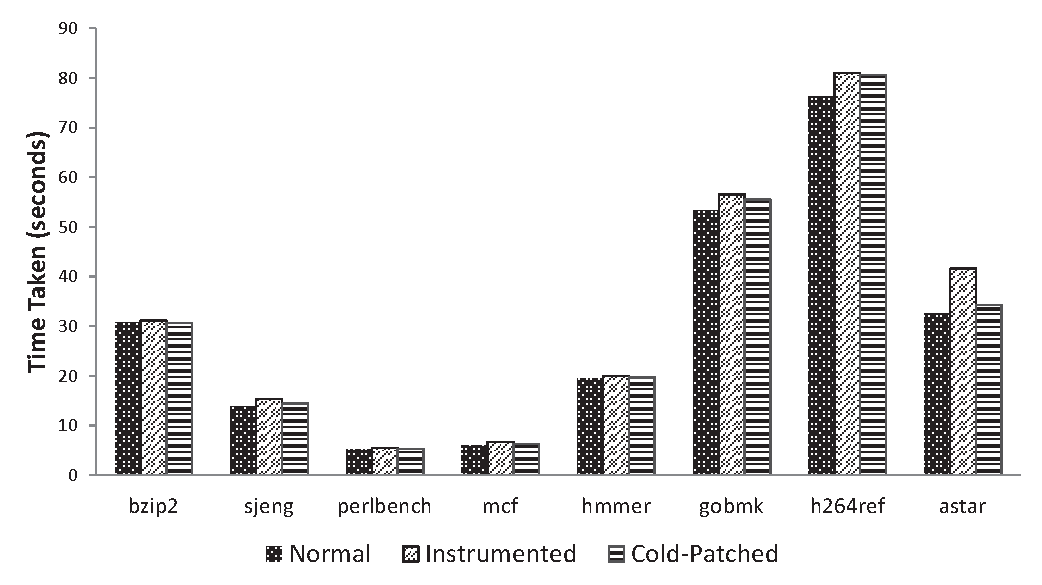
\includegraphics[width=0.8\textwidth]{iprobe/Images/OverheadCold.eps}
    \caption{Overhead of iProbe ``ColdPatch Stage" on SPEC CPU 2006 Benchmarks.}
    \label{fig:overhead_table}
  \end{center}
\end{figure}


\subsection{Overhead of HotPatching and Scalability Analysis}

%One of the advantages of iProbe is that it scales extremely well.
We compared iProbe with UTrace (User Space Tracing in SystemTap) \cite{utrace}, and DynInst \cite{dyninst} on a x86\_64, dual-core machine with Ubuntu 12.10 kernel. 
To test the scalability of these tools, we designed a micro-benchmark and tested the overhead for an increasing amount of events instrumented. 
We instrumented a dummy application with multiple calls to an empty function \texttt{foo}, the instrumentation function in the cases simply increases a global counter for each event triggered (entry and exit of foo). 
Tools were written using all three frameworks to instrument the start and end of the target function and call the instrumentation function. 

Figure \ref{fig:scalability} shows our results when applying iProbe and SystemTap on this micro-benchmark. 
To test the scalability of our the tools, we have increased the number of calls made to \texttt{foo} exponentially (increase by multiples of 10). 
We found that iProbe scales very well and is able to keep the overhead to less than five times for millions of events (10\textsuperscript{8}) generated in less than a second (normal execution) for entry as well as exit of the function. 
While iProbe executed in 1.5 seconds, the overhead observed in SystemTap is around 20 minutes for completion of a subsecond execution, while DynInst takes about 25 seconds. 

As explained in Section \ref{sec:trampoline}, tools such as DynInst use a trampoline mechanism, hence have a minimum of 2 call instructions for each instrumentation.
Additionally SystemTap uses a context switch to switch to the kernel space over and above the traditional trampoline mechanism, resulting in the high overhead, and less scalability observed in our results.

\begin{figure}[h!]
  \begin{center}
    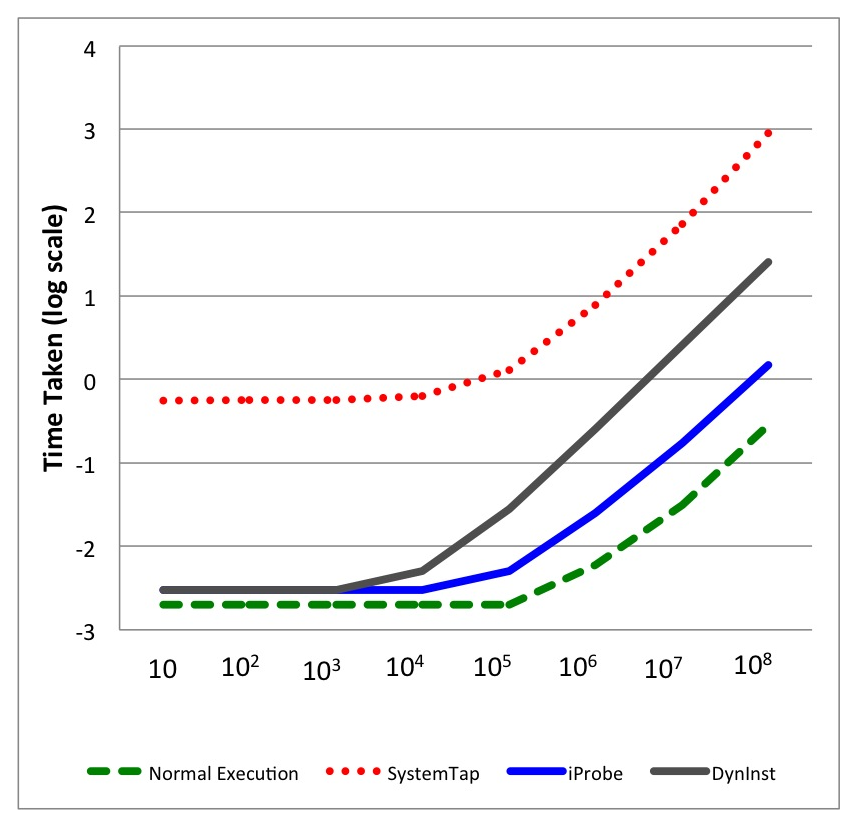
\includegraphics[width=0.8\textwidth]{iprobe/Images/scalability.eps}
    \caption{Overhead and Scalability Comparison of iProbe HotPatching vs. SystemTap vs. DynInst using a Micro-benchmark.}
    \label{fig:scalability}
  \end{center}
\end{figure}

%
%\begin{table}[h]
%\begin{center}
%    \begin{tabular}{ | l | l | l | l|}
%    \hline
%    No. of Events & Normal & SystemTap & iProbe \\ \hline
%    10 & 0.002 & 0.556 & 0.002 \\ \hline
%    10\textsuperscript{2} & 0.002 & 0.566 & 0.003 \\ \hline
%    10\textsuperscript{3} & 0.002 & 0.56 & 0.003 \\ \hline
%   	10\textsuperscript{4} & 0.002 & 0.624 & 0.003 \\ \hline
%    10\textsuperscript{5} & 0.002 & 1.276 & 0.005  \\ \hline
%    10\textsuperscript{6} & 0.007 & 7.805 & 0.025 \\ \hline
%    10\textsuperscript{7} & 0.031 & 72.91 & 0.174 \\ \hline
%    10\textsuperscript{8} & 0.281 & 1200 & 1.502 \\ \hline
%    \end{tabular}
%\end{center}
%    \label{tab:scaling}
%    \caption{A scalability comparison of iProbe vs SystemTap using a micro-benchmark}
%\end{table}


%\begin{table}[h]
%\begin{center}
%    \begin{tabular}{ | l | l | p{2cm} | p{2cm}|}
%    \hline
%    Name & Time & Instrumentation Points & Number of Events \\ \hline
%    bzip2 & 30.7 & 31.2 & 30.7 \\ \hline
%     & 13.8 & 15.4 & 14.4 \\ \hline
%     & 5.24 & 5.49 & 5.24 \\ \hline
%     & 5.98 & 6.72 & 6.28 \\ \hline
%     & 19.5 & 20 & 19.7  \\ \hline
%     & 3.8 & 3.8 & 3.8 \\ \hline
%     & 53.4 & 53.4 & 53.4 \\ \hline
%     & 0.303 & 20 & 19.7  \\ \hline
%     & 76.3 & 3.8 & 3.8 \\ \hline
%     & 1.93 & 53.4 & 53.4 \\ \hline
%     & 30.6 & 20 & 19.7  \\ \hline
%     & 0.936 & 3.8 & 3.8 \\ \hline
%    \end{tabular}
%\end{center}
%\label{tab:RealOverhead}
%\caption{\textbf{Overhead when HotPatching with SPEC CPU 2006 benchmark}}
%\end{table}

